\documentclass[9pt,a4paper,twocolumn,twoside]{rho-class/rho}

% --- 1. Idioma y matemáticas básicas ---
\usepackage[spanish,es-nodecimaldot,es-noindentfirst,es-noshorthands]{babel}


% --- 2. EL TRUCO DE MAGIA (BIEN ESCRITO) ---
% Borramos los comandos problemáticos usando su nombre exacto interno
\expandafter\let\csname not=\endcsname\relax
\expandafter\let\csname not<\endcsname\relax
\expandafter\let\csname not>\endcsname\relax

% Ahora ya podemos cargar la fuente moderna sin que explote
\usepackage{fontspec}
\usepackage{unicode-math}
% --- 3. Bibliografía ---
\addbibresource{rho.bib}

% --- 4. Datos del Informe ---
\title{Estudio de la sección eficaz de producción de pares top-antitop en colisiones protón-protón a $\sqrt{s} = 7$ TeV con el detector CMS}
\author{Edgar Fernández Vigil}
\affil{Física - Facultad de Ciencias - Universidad de Oviedo}
\dates{\today}
\journalname{FAEA - Práctica de Laboratorio}
\journal{$t\bar{t}$ \ a \ $\sqrt{s} = 7$ TeV}

% --- 5. Resumen ---
\begin{abstract}
En este iforme se detalla el análisis realizado para medir la sección eficaz de producción de pares top-antitop en colisiones protón-protón a una energía de $\sqrt{s} = 7$ TeV utilizando datos del detector CMS. Se describen los criterios de selección de eventos, la estimación de fondos, y la extracción de la señal. Finalmente, se presenta el resultado obtenido para la sección eficaz y su comparación con predicciones teóricas.
\end{abstract}
% ----------------------------------------------------------
\begin{document}

    \maketitle
    \thispagestyle{firststyle}

\section{Introducción}

\rhostart{L}a sección eficaz de producción de pares top-antitop es una cantidad fundamental en la física de partículas, ya que proporciona información crucial sobre la interacción fuerte y el modelo estándar.

En este caso estaremos analizando datos de colisiones protón-protón a una energía de $\sqrt{s} = 7$ TeV, obtenidos por el detector CMS en el LHC. El objetivo principal es medir la sección eficaz de producción de pares top-antitop y compararla con las predicciones teóricas.

A primer orden en teoría de perturbaciones, los diagramas de Feynman que contribuyen a este proceso son la fusión de gluones, con cerca de un $80\%$ de la contribucióntotal, y la aniquilación quark-antiquark , con el $20\%$.

\begin{figure}[H]
    \centering
    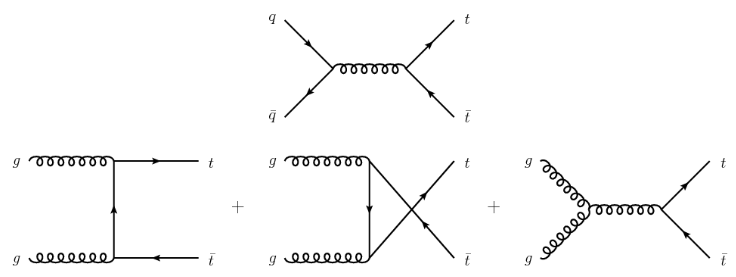
\includegraphics[width=0.9\columnwidth]{img/Feynman_produccion_top_antitop.png}
    \caption{Diagrama de Feynman del proceso de producción de pares top-antitop.}
    \label{fig:Feynman_produccion_top_antitop}
\end{figure}

Primeramente debemos definir el canal de desintegración que vamos a estudiar. Dadas las características del detector y su capacidad para identificar leptones (especialmente muones) y reconstruir jets con alta precisión, nos centraremos en el que un W decae en un muon y un neutrino, mientras que el otro W decae en dos quarks. Este canal es conocido como el canal semileptónico.

Por lo tanto, los productos de la desintegración que esperamos observar en el detector son:
\begin{itemize}
    \item \textbf{Un muon} de alta energía proveniente de la desintegración del W.
    \item \textbf{Un neutrino}, que no interactúa con el detector y se manifestará como energía faltante (MET).
    \item \textbf{Dos jets} provenientes de la hadronización de los quarks del otro W.
    \item \textbf{Dos jets adicionales} provenientes de la hadronización de los quarks b del top y antitop (b-jets).
\end{itemize}

Existe otro canal de desintegración, el dileptónico, donde ambos W decaen en leptones (por ejemplo, dos muones), pero este canal tiene una tasa de eventos más baja y es más difícil de analizar debido a la presencia de dos neutrinos. Pero este canal es que que mejores medidas de la sección eficaz ha proporcionado, por lo que es un canal muy estudiado.

\begin{figure}[H]
    \centering
    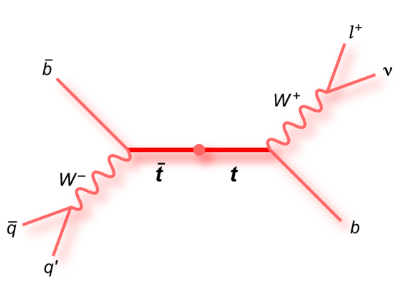
\includegraphics[width=0.75\columnwidth]{img/Feynman_desintegracion_top_antitop.png}
    \caption{Diagrama de Feynman del proceso de desintegración de un par top-antitop en el canal semileptónico.}
    \label{fig:Feynman_desintegracion_top_antitop}
\end{figure}

Además dada la producción de pares top-antitop, también se pueden producir otros procesos que pueden imitar la señal que estamos buscando, como la producción de W+jets o la producción de pares de bosones WZ. Por lo tanto, debemos de estudiar cuidadosamente loa fondos que pueden contribuir a nuestra muestra de eventos, estudiando a partir de simulaciones de Monte Carlo y aplicando criterios de selección que nos permitan maximizar la señal y minimizar los fondos, sin perder demasiados eventos de señal.

Todos los datos que hemos usado durante la práctica han sido los siguientes:
\begin{itemize}
    \item \textbf{Datos reales:} Datos extraidos de colisiones protón-protón a $\sqrt{s} = 7$ TeV, correspondientes a una luminosidad integrada de $50.0 \, \mathrm{pb}^{-1}$, recolectados por el detector CMS durante el año 2011.
    \item \textbf{Simulaciones de producción y recostrucción de MC:} Simulaciones de Monte Carlo para la producción y recostrucción de eventos de pares top-antitop, y para el fondo (W+jets, WZ, WW, ZZ, Drell-Yan, single top, QCD) todas a $1 \mathrm{pb}^{-1}$.
\end{itemize}

\begin{figure}[H]
    \centering
    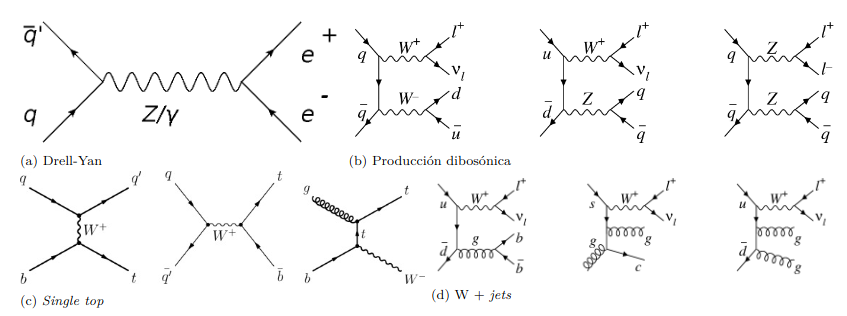
\includegraphics[width=1.0\columnwidth]{img/Feynman_fondo.png}
    \caption{Diagramas de Feynman de los procesos de fondo.}
    \label{fig:Feynman_fondo}
\end{figure}

\section{Metodología}

Ya hemos definido el proceso que queremos estudiar, el canal de desintegración y los datos que vamos a usar, ahora debemos definir la metodología que vamos a seguir para realizar el análisis.
\subsection{Selección de eventos}

Para seleccionar los eventos que corresponden al proceso de producción de pares top-antitop en el canal semileptónico, aplicaremos una serie de criterios de selección basados en las características de los productos de la desintegración que esperamos observar en el detector. Estos criterios son:
\begin{itemize}
    \item Presencia de un único muon de alta energía con $p_T > 28$ GeV y $|\eta| < 2.4$.
    \item Presencia de al menos 3 jets con $p_T > 30$ GeV y $|\eta| < 2.4$, de los cuales al menos uno deben ser identificados como b-jets.
    \item Presencia de energía faltante (MET) mayor a 20 GeV, para indicar la presencia del neutrino.
    \item Que no exista presencia de electrones
\end{itemize}

Estos criterios no son elegidos al azar, sino que se basan en estudios previos de las simulaciones de Monte Carlo, donde se ha observado que estos cortes permiten maximizar la señal y minimizar los fondos. Además, estos criterios son consistentes con las capacidades del detector CMS para identificar muones, jets y medir el MET, ya que por ejemplos cortes como en la pseudorapidez son derivados de las propias limitaciones geometricas del detector. Otros cortes, como el de numero de jets, nos asegura minimizar el fondo de los fondos más significativos, sin reducir en exceso la señal. Por ejemplo, el corte en el número de jets nos ayuda a reducir el fondo de W+jets, que es uno de los fondos más importantes en este análisis, ya que este proceso puede producir un muon y MET similar a nuestra señal, pero generalmente produce menos jets que el proceso de producción de pares top-antitop (basado en \cite{cms2013ttbar_ljets}).

Además no podemos aplicar cortes a discreción, menos datos también se traducen en una mayor incertidumbre estadística, por lo que debemos de encontrar un equilibrio entre maximizar la señal y minimizar los fondos, sin perder demasiados eventos de señal.

\subsection{Eficiencias}

Sabemos que en el CERN se producen un monton de eventos cada muy poco tiempo, y se las han ideado para gestionar esta ingente cantidad de datos aplicando una serie de filtros a nivel de hardware y software, conocidos como triggers, que permiten seleccionar los eventos más interesantes para su análisis posterior. En nuestro caso, el trigger que se ha utilizado para recolectar los datos es un trigger que requiere la presencia de un muon con $p_T > 24$ GeV, pero desgraciadamente este trigger no es perfecto, y no selecciona todos los eventos que cumplen con esta condición, por lo que debemos de corregir nuestra medida de la sección eficaz por la eficiencia del trigger, inicialmente haremos un estudio de la eficiencia del mismo, ya que sería lógico aplicar un corte sobre el que el trigger comienza a ser lo suficientemente efectivo.

Esta no es la única eficiencia que debemos de tener en cuenta, entre otras eficiencias la más reseñable quizás sea la de la identificación de b-jets, ya que es un criterio de selección fundamental para nuestro análisis, y esta eficiencia no es perfecta, por lo que también debemos de corregir nuestra medida de la sección eficaz por la eficiencia de identificación de b-jets.

Estas eficiencias se pueden estimar a partir de las simulaciones de Monte Carlo, de donde extraeremos la información necesaria para calcular estas eficiencias, y aplicaremos las correcciones correspondientes a nuestra medida de la sección eficaz. Además, también debemos de tener en cuenta las incertidumbres asociadas a estas eficiencias, ya que estas incertidumbres se traducen en una mayor incertidumbre en nuestra medida de la sección eficaz.

Por ejemplo la eficiencia de b-tagging también nos obliga a corregir los pesos de los eventos en las simulaciones de Monte Carlo, ya que estos eventos se generan con una eficiencia de b-tagging diferente a la que se observa en los datos reales, por lo que debemos de aplicar un factor de corrección a los pesos de los eventos en las simulaciones de Monte Carlo para que estos reflejen la eficiencia de b-tagging observada en los datos reales.

Entonces los criterios para el cálculo de las eficiencias son los siguientes:
\begin{itemize}
    \item Haremos primero un estudio de la eficiencia del trigger, para determinar a partir de qué valor de $p_T$ el trigger es lo suficientemente eficiente, y aplicaremos un corte sobre este valor para asegurar que estamos trabajando en una región donde el trigger es eficiente.
    la eficiencia entonces se calculará como (independientes de la selección de eventos):

    \begin{equation}
        \epsilon_{\text{trigger}} = \frac{N_{\text{eventos que pasan el trigger}}}{N_{\text{eventos totales}}}
    \end{equation}

    \item Para la eficiencia de identificación de b-jets, utilizaremos únicamente eventos de Monte Carlo a de pares top-antitop, ya que estos eventos contienen b-jets reales, y calcularemos la eficiencia como
    
    \begin{equation}
        \epsilon_{\text{b-tag}} = \frac{N_{\text{b-jets identificados correctamente}}}{N_{\text{b-jets totales}}}
    \end{equation}
    
    donde dotaremos de b-jets a los jets que cumplan con la condición de que su $\Delta R$ sea menor que 0.3. Así los que están bien identificados serán aquellos que cumplan con esta condición y además sean identificados como b-jets por el algoritmo de b-tagging, donde nostros hemos escogido como score mínimo un valor de 2.0, asegurandonos que el algoritmo de b-tagging es lo suficientemente estricto para minimizar el número de falsos positivos, pero sin ser tan estricto como para perder demasiados eventos de señal.

    \item Por último incluiremos también la eficiencia de recostrucción de los muones $\epsilon_{\mu} = 0.99$
\end{itemize}

\subsection{Aceptancia}

Dados todos los cortes y eficiencias que hemos aplicado si nos pusiesemos a calcular la sección eficaz sin tener en cuenta la aceptancia, estaríamos cometiendo un error, ya que no todos los eventos de producción de pares top-antitop cumplen con los criterios de selección que hemos definido, por lo que debemos de corregir nuestra medida de la sección eficaz por la aceptancia del proceso, que se define como la fracción de eventos de producción de pares top-antitop que cumplen con los criterios de selección definidos. Es decir estamos calculando la sección eficaz de que se produzca un par top-antitop y sus productos de desintegración cumplan con los criterios de selección, pero lo que realmente queremos es la sección eficaz total de producción de pares top-antitop, por lo que debemos de corregir nuestra medida.

Entonces sobre nuestra simulación de Monte Carlo, a nivel de generación, debemos de establecer una región fiducial, es decir, como ya tenemos los productos y sus energías, establecer cuales de ellos cumplirán con el criterio de selección, y si dividivos la cantidad de eventos de la región fiducial entre la cantidad total obtendremos la aceptancia del proceso.

\begin{equation}
    A = \frac{N_{\text{eventos en la región fiducial}}}{N_{\text{eventos totales}}}
\end{equation}

\subsection{Calculo de la sección eficaz}

Una vez que hemos aplicado todos los criterios de selección, corregido por las eficiencias y la aceptancia, ya podemos proceder a calcular la sección eficaz de producción de pares top-antitop utilizando la siguiente fórmula:

\begin{equation}
    \sigma_{t\bar{t}} = \frac{N_{\text{eventos seleccionados}} - N_{\text{eventos de fondo}}}{\mathcal{L} \cdot A \cdot \epsilon_{\text{total}}}
\end{equation}

Donde $N_{\text{eventos seleccionados}}$ es el número de eventos que cumplen con los criterios de selección, $N_{\text{eventos de fondo}}$ es el número de eventos que corresponden a procesos de fondo que también cumplen con los criterios de selección, $\mathcal{L}$ es la luminosidad integrada de los datos, $A$ es la aceptancia del proceso, y $\epsilon$ es la eficiencia total del proceso que se calcula como

\begin{equation}
    \epsilon_{\text{total}} = \epsilon_{\text{trigger}} \cdot \epsilon_{\text{b-tag}} \cdot \epsilon_{\mu}
\end{equation}

\subsection{Incertidumbres}

Como para cualquier medida experimental, es fundamental estimar las incertidumbres asociadas a nuestra medida de la sección eficaz, ya que estas incertidumbres nos permiten conocer la precisión de nuestra medida y compararla con las predicciones teóricas. La incertidumbre final se reporta separada en tres contribuciones: estadística, luminosidad y sistemática. La parte estadística se toma a partir de la fluctuación Poisson del numerador, que en la práctica se extrae de los histogramas:

\begin{equation}
    \delta N_{\mathrm{obs}} = \sqrt{N_{\mathrm{obs}}},
\end{equation}

\begin{equation}
    \delta \sigma_{\mathrm{stat}} = \frac{\delta N_{\mathrm{obs}}}{\mathcal{L}\,A\,\epsilon_{\mathrm{tot}}}
    = \sigma_{t\bar{t}}^{\mathrm{nom}}\,\frac{\sqrt{N_{\mathrm{obs}}}}{N_{\mathrm{obs}} - N_{\mathrm{bkg}}}.
\end{equation}

La parte sistemática se evalúa variando de forma independiente cada fuente por su incertidumbre y recalculando la sección eficaz en ambos sentidos. Para una fuente $i$ con variación $\delta_i$, definimos

\begin{equation}
    \sigma_i^{\pm} = \frac{N_{\mathrm{obs}} - \left(N_{\mathrm{bkg}} \pm \delta_i\right)}{\mathcal{L}\,A\,\epsilon_{\mathrm{tot}}},
\end{equation}

\begin{equation}
    \Delta_i = \max\left(\left|\sigma_i^{+} - \sigma_{t\bar{t}}^{\mathrm{nom}}\right|,\,\left|\sigma_i^{-} - \sigma_{t\bar{t}}^{\mathrm{nom}}\right|\right).
\end{equation}

Para las incertidumbres de normalización de los fondos usamos $\delta_i = f_i\,N_i$, con $f_i$ igual a 50\% para $W+$jets, 100\% para QCD, 50\% para $WW$, $WZ$ y $ZZ$, 15\% para Drell-Yan y 30\% para single-top. Para las eficiencias y la luminosidad se toma

\begin{equation}
    \epsilon_b^{\pm} = \epsilon_b\left(1 \pm 0.10\right), \qquad
    \mathcal{L}^{\pm} = \mathcal{L}\left(1 \pm 0.10\right), \qquad
    \epsilon_{\mathrm{tr}}^{\pm} = \epsilon_{\mathrm{tr}} \pm \frac{1-\epsilon_{\mathrm{tr}}}{2}.
\end{equation}

Analogamente a las fuentes sistemáticas, se varía cada uno de estos parámetros en ambos sentidos y se recalcula la sección eficaz, obteniendo así $\Delta_b$, $\Delta_{\mathcal{L}}$ y $\Delta_{\mathrm{tr}}$ como diferencia respecto al valor nominal.La incertidumbre de la aceptancia se deriva a partir de la estadística del numerador y del denominador,

\begin{equation}
    A = \frac{N_{\mathrm{fid}}}{N_{\mathrm{gen}}},
\end{equation}

\begin{equation}
    \delta A = A\,\sqrt{\left(\frac{\delta N_{\mathrm{fid}}}{N_{\mathrm{fid}}}\right)^2 + \left(\frac{\delta N_{\mathrm{gen}}}{N_{\mathrm{gen}}}\right)^2},
\end{equation}

tomando $\delta N_{\mathrm{fid}} \simeq \sqrt{N_{\mathrm{fid}}}$ y, si $N_{\mathrm{gen}}$ se considera fijo, $\delta N_{\mathrm{gen}} = 0$. La incertidumbre de reconstrucción de muones fue dada en el apartado anterior.

Finalmente, la incertidumbre sistemática total se obtiene combinando en cuadratura todas las contribuciones,

\begin{equation}
    \delta \sigma_{\mathrm{syst}} = \sqrt{\sum_i \Delta_i^2},
\end{equation}

suponiendo que no existe correlación entre las distintas fuentes de incertidumbre.

La incertidumbre total de la medida se obtiene combinando en cuadratura las tres contribuciones anteriores:

\begin{equation}
    \delta \sigma_{\mathrm{tot}} = \sqrt{\delta \sigma_{\mathrm{stat}}^2 + \delta \sigma_{\mathcal{L}}^2 + \delta \sigma_{\mathrm{syst}}^2}.
\end{equation}

Así, el resultado final de la sección eficaz se expresa como

\begin{equation}
    \sigma_{t\bar{t}} = \sigma_{t\bar{t}}^{\mathrm{nom}} \pm \delta \sigma_{\mathrm{stat}} \pm \delta \sigma_{\mathcal{L}} \pm \delta \sigma_{\mathrm{syst}},
\end{equation}

Con la incertidumbre total $\delta \sigma_{\mathrm{tot}}$ dada por la combinación en cuadratura anterior.

\section{Resultados}

Comenzando con los resultados lo primero que debemos de ver es la Eficiencia del trigger, en el rango de 20 a 30 GeV, que es el rango donde el trigger comienza a ser eficiente, y vemos que a partir de los 28 GeV el trigger es lo suficientemente eficiente, por lo que aplicaremos un corte sobre este valor para asegurar que estamos trabajando en una región donde el trigger es eficiente.

\begin{figure}[H]
    \centering
    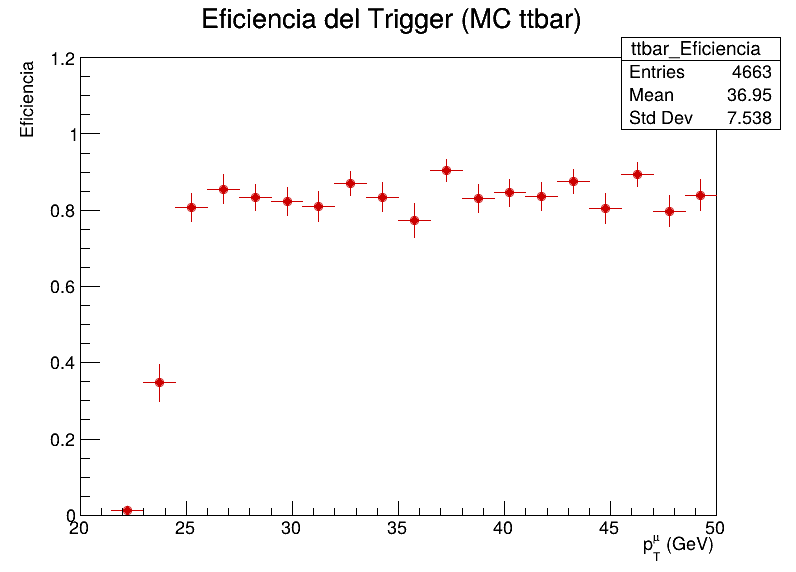
\includegraphics[width=0.9\columnwidth]{results/Eficiencia.png}
    \caption{Eficiencia del trigger en función del $p_T$ del muon.}
    \label{fig:eficiencia_trigger}
\end{figure}

Esta gráfica esta hecha solo para $t\bar{t}$ ya que es el único que recoge eventos que no hayan pasado el trigger, por lo que es el único que nos permite calcular la eficiencia del trigger.

Vemos que cerca de los 24 GeV empieza a crecer la eficiencia, ya que es el valor de construcción, y empieza a ser lo suficientemente eficiente a partir de los 28 GeV, por lo que aplicaremos un corte sobre este valor para asegurar que estamos trabajando en una región donde el trigger es eficiente.

los siguientes cortes se aplican para reducir la cantidad de eventos de fondo, siendo los ya descritos, dejandonos una distribución de eventos donde veremos una clara predominancia de la región de señal, ya que de forma inteligente por ejemplo con los cortes de al menos 3 jets estamos eliminando gran parte del fondo de W+jets, que es uno de los fondos más importantes en este análisis, ya que este proceso puede producir un muon y MET similar a nuestra señal, pero generalmente produce menos jets que el proceso de producción de pares top-antitop.

Además exigir al menos 1 b-jet nos ayuda a reducir el fondo, podríamos pensar que si exigimos 2 lo tenemos todo hecho, pero nos reduce abruptamente la región de señal, aumentando la incertidumbre estadística de nuestra medida, llegando a reducir la muestra incluso a 20 eventos, por lo que hemos decidido ser más conservadores con respecto a los cortes. Por otro lado el de la MET nos ayuda a reducir el fondo de QCD, que es otro de los fondos más importantes en este análisis, ya que este proceso puede producir un muon y jets similar a nuestra señal, pero generalmente no produce MET, por lo que un corte en el MET nos ayuda a reducir este fondo.

\begin{figure}[H]
    \centering
    
    % --- PRIMERA FILA ---
    % Imagen 1 (Arriba Izquierda)
    \begin{subfigure}[b]{0.24\textwidth}
        \centering
        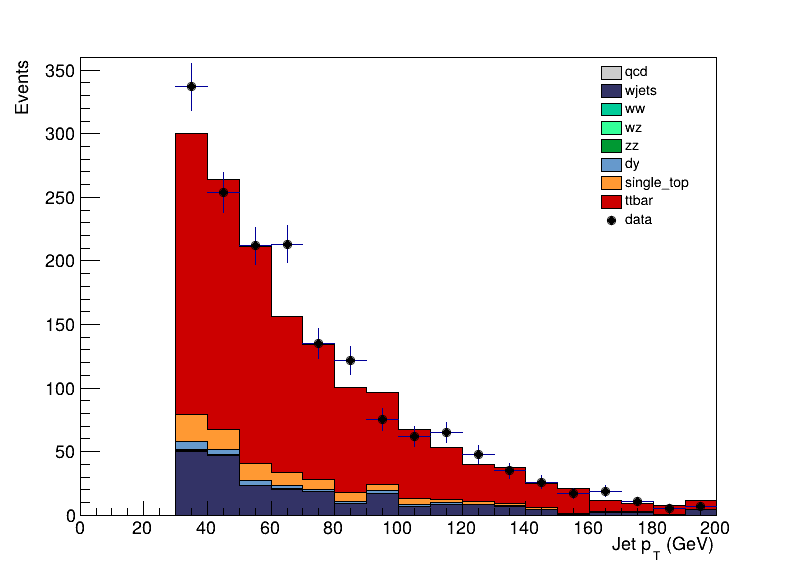
\includegraphics[width=\textwidth]{results/JetPt.png}
        \caption{Jet $p_T$}
        \label{fig:img1}
    \end{subfigure}
    \hfill % Esto añade espacio horizontal entre las dos imágenes
    % Imagen 2 (Arriba Derecha)
    \begin{subfigure}[b]{0.24\textwidth}
        \centering
        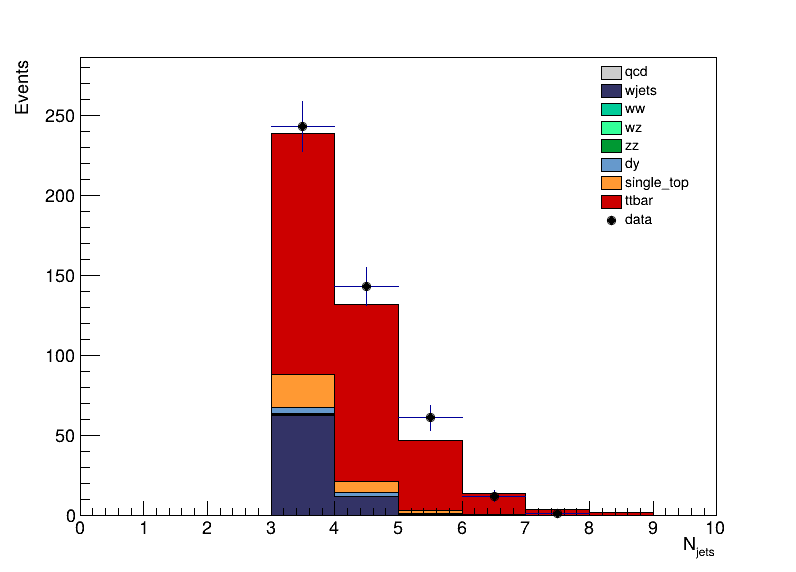
\includegraphics[width=\textwidth]{results/NJet.png}
        \caption{Número de jets}
        \label{fig:img2}
    \end{subfigure}
    
    \vspace{0.5cm} % Espacio vertical entre la primera y la segunda fila
    
    % --- SEGUNDA FILA ---
    % Imagen 3 (Abajo Izquierda)
    \begin{subfigure}[b]{0.24\textwidth}
        \centering
        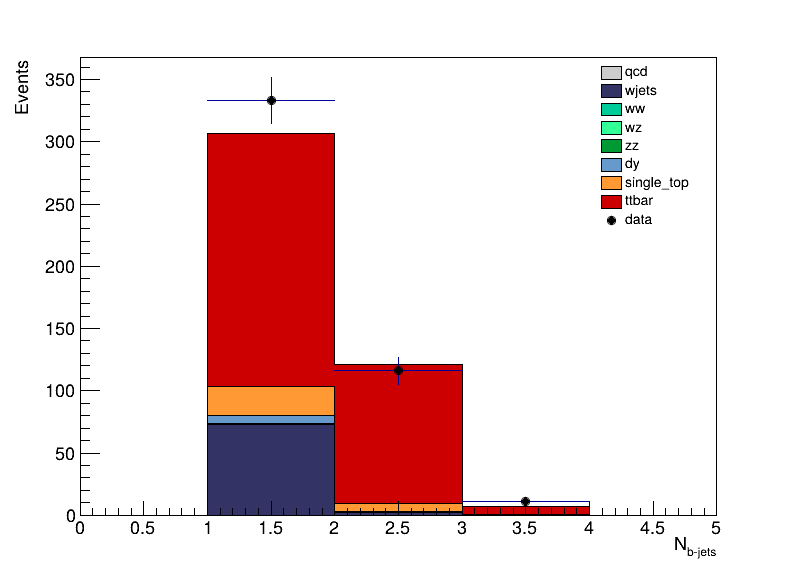
\includegraphics[width=\textwidth]{results/NbJets.png}
        \caption{Número de b-jets}
        \label{fig:img3}
    \end{subfigure}
    \hfill
    % Imagen 4 (Abajo Derecha)
    \begin{subfigure}[b]{0.24\textwidth}
        \centering
        
\includegraphics[width=\textwidth]{results/MuonPt.png}
        \caption{Muon $p_T$}
        \label{fig:img4}
    \end{subfigure}
    \begin{subfigure}[b]{0.24\textwidth}
        \centering
        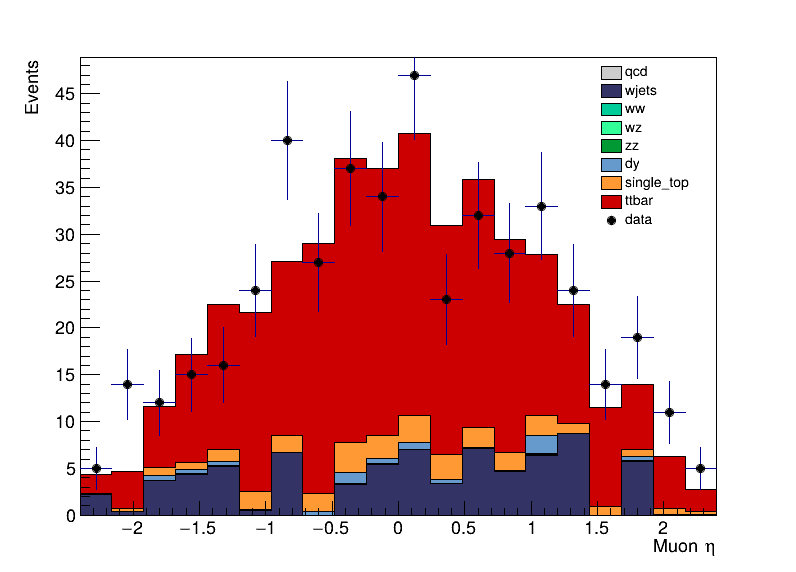
\includegraphics[width=\textwidth]{results/MuonEta.png}
        \caption{Muon $\eta$}
        \label{fig:img5}
    \end{subfigure}
    \hfill % Esto añade espacio horizontal entre las dos imágenes
    % Imagen 2 (Arriba Derecha)
    \begin{subfigure}[b]{0.24\textwidth}
        \centering
        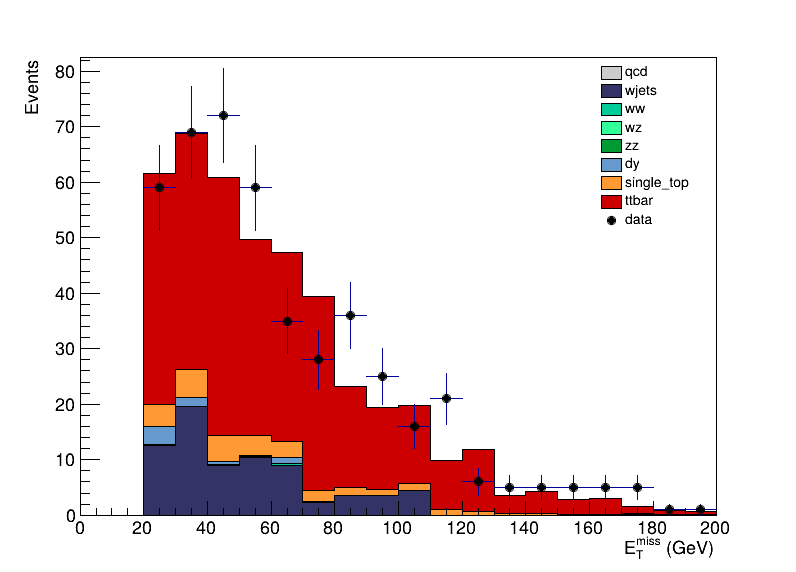
\includegraphics[width=\textwidth]{results/MET.png}
        \caption{MET}
        \label{fig:img6}
    \end{subfigure}
    
    \vspace{0.5cm} % Espacio vertical entre la primera y la segunda fila
    
    
    % Título y etiqueta de toda la figura en conjunto
    \caption{Resumen global de los histogramas.}
    \label{fig:figura_global}
\end{figure}

Aunque podamos observar discrepancias entre los datos y la reconstrucción esta claro que se mantiene cierta tendencia, y que la región de señal es claramente predominante, lo que nos permite realizar una medida de la sección eficaz con una incertidumbre razonable. Además, estas discrepancias pueden ser debidas a una mala modelización de los fondos, o a una mala modelización de las eficiencias, por lo que es importante tener en cuenta estas posibles fuentes de incertidumbre a la hora de interpretar los resultados.

Tras aplicar todos los cortes y correcciones, obtenemos una medida de la sección eficaz de producción de pares top-antitop en colisiones protón-protón a $\sqrt{s} = 7$ TeV de:

\begin{equation}
    \sigma_{t\bar{t}} = 221.15 \pm 13.75 \, (\mathrm{stat}) \pm 37.47 \, (\mathrm{syst}) \pm 20.10 \, (\mathcal{L}) \, \mathrm{pb}
\end{equation}
\vspace{0.05cm}

Vemos que la incertidumbre sistemática es la más grande de las tres, lo que indica que la principal limitación de nuestra medida es la comprensión de los fondos y las eficiencias, por lo que sería importante realizar un estudio más detallado de estas fuentes de incertidumbre para mejorar la precisión de nuestra medida. Además, esta medida es consistente con las predicciones teóricas del modelo estándar, que predice una sección eficaz de producción de pares top-antitop a $\sqrt{s} = 7$ TeV de aproximadamente 172 pb, por lo que podemos concluir que nuestra medida es consistente con el modelo estándar y que no se observa ninguna desviación significativa, ya que la predicción del modelo estándar se encuentra dentro del rango de incertidumbre de nuestra medida.

Más alla de la medida de la sección eficaz, podemos tabular todos los valores obtenidos:

\begin{table}[hbt!]
    \centering
    \begin{tabular}{|l|c|}
        \hline
        Variables & Valores \\
        \hline
        Luminosidad integrada ($\mathcal{L}$)  & $50.0 \, \mathrm{pb}^{-1}$ \\
        \hline
        Aceptancia (A)  & $0,0754$ \\
        \hline
        Eficiencia trigger ($\epsilon_{\text{trigger}}$)  & $0.8181$ \\
        \hline
        Eficiencia b-tagging ($\epsilon_{\text{b-tag}}$)  & $0.8181$ \\
        \hline
        Eficiencia total  & $0.4152$ \\
        \hline
        $N_{\text{obs}}$  & $456$ \\
        \hline
        $N_{\text{fondo}}$  & $112$ \\
        \hline
        Eventos netos de Señal  & $343$ \\
        \hline
        Señal Expected & $321$ \\
        \hline
    \end{tabular}
\end{table}

Todo se encuentra dentro del rango esperado, obteniendo quizás valores bajos para la eficiencia de b-tagging, pero esto se debe a que hemos escogido un score mínimo de 2.0, asegurandonos que el algoritmo de b-tagging es lo suficientemente estricto para minimizar el número de falsos positivos, pero sin ser tan estricto como para perder demasiados eventos de señal.

\section{Discusión y conclusiones}
En este informe se ha detallado el análisis realizado para medir la sección eficaz de producción de pares top-antitop en colisiones protón-protón a $\sqrt{s} = 7$ TeV utilizando datos del detector CMS. Se han descrito los criterios de selección de eventos, la estimación de fondos, y la extracción de la señal. Finalmente, se ha presentado el resultado obtenido para la sección eficaz y su comparación con predicciones teóricas.

La medida obtenida para la sección eficaz de producción de pares top-antitop es consistente con las predicciones teóricas del modelo estándar, lo que indica que no se observa ninguna desviación significativa y que el modelo estándar sigue siendo una descripción válida de la física de partículas a estas energías. Sin embargo, la incertidumbre sistemática es la principal limitación de nuestra medida, lo que sugiere que sería importante realizar un estudio más detallado de las fuentes de incertidumbre asociadas a los fondos y las eficiencias para mejorar la precisión de nuestra medida. Además, sería interesante comparar esta medida con otras medidas de la sección eficaz de producción de pares top-antitop realizadas por otros experimentos, como ATLAS, para verificar la consistencia de los resultados y obtener una medida más precisa de la sección eficaz de producción de pares top-antitop a $\sqrt{s} = 7$ TeV.

Incluso quizás más datos nos ayudaría a aplicar cortes más estrictos sin tener la preocupación de perder demasiados eventos de señal, lo que nos permitiría reducir aún más la cantidad de eventos de fondo y mejorar la precisión de nuestra medida. Además, con más datos podríamos realizar un estudio más detallado de las distribuciones de las variables cinemáticas de los productos de desintegración, lo que nos permitiría obtener una mejor comprensión del proceso de producción de pares top-antitop y sus características.

Cabe destacar una curiosidad encontrada durante el análisis, tal y como se comentaba en el guión la eficiencia del b-tagging depende de los cortes de selección, cosa en la que Jorge estaba en desacuerdo, y es lógico pensar que la eficiencia debería de ser independiente de los cortes de selección, aún así haciendo la prueba calculando la eficiencia de b-tagging únicamente sobre sucesos que pasen los cortes el resultado de la sección eficaz era de $175 pb$, reduciendo un poco la incertidumbre sistemática. Finalmente a pesar de esto hemos decidido quedarnos con la otra por ser más consistente en cuanto a como definimos eficiencias.

\nocite{*}

\printbibliography

\end{document}


\begin{table}[hbt!]
    \centering
    \begin{tabular}{lc}
        \hline
        n & $e$ ($10^{-19}$ C) \\
        \hline
        gota 1  & $1.79 \pm 0.05$ \\
        gota 2  & $1.89 \pm 0.05$ \\
        gota 3  & $1.61 \pm 0.03$ \\
        gota 4  & $1.60 \pm 0.03$ \\
        gota 5  & $1.50 \pm 0.03$ \\
        gota 6  & $2.11 \pm 0.10$ \\
        gota 7  & $1.82 \pm 0.03$ \\
        gota 8  & $1.93 \pm 0.10$ \\
        gota 9  & $2.31 \pm 0.10$ \\
        gota 10 & $2.48 \pm 0.10$ \\
        gota 11 & $1.59 \pm 0.03$ \\
        gota 12 & $1.58 \pm 0.03$ \\
        gota 13 & $1.64 \pm 0.10$ \\
        gota 14 & $1.76 \pm 0.05$ \\
        gota 15 & $1.71 \pm 0.02$ \\
        gota 16 & $1.73 \pm 0.10$ \\
        \hline
    \end{tabular}
    \vspace{0.1cm}
\caption{Valor estimado de la carga elemental ($e$) para cada gota}
\label{tab:carga_elemental_gotas}
\end{table}

\begin{figure}[H]
    \centering
    
\includegraphics[width=0.7\columnwidth]{img/planteamiento-teorico-carga-elec.png}
    \caption{Planteamiento teórico del balance de fuerzas.}
    \label{fig:planteamiento-teorico-carga-elec}
\end{figure}